\chapter{THỬ NGHIỆM VÀ ĐÁNH GIÁ}
\section{Triển khai chạy thử nghiệm trên cloud}
Trong đồ án này, chúng tôi sử dụng Microsoft Azure làm nhà cung cấp dịch vụ
cloud và sử dụng Azure Kubernetes Service
để triển khai các server~\cite{kubeazure:online}.
Kiến trúc tổng quan của hệ thống như hình sau:
\begin{figure}[H]
\centering
\includegraphics[width=10cm]{images/architecture.png}
\caption{Kiến trúc tổng quan của hệ thống}
\end{figure}
Trong đó:
\begin{itemize}[topsep=0ex]
\item Nginx: sử dụng để làm web server trả về các file tĩnh html và js khi
ứng dụng được mở lên lần đầu, đồng thời được sử dụng làm Reverse Proxy đến
Golang Server cho các REST API.

\item Golang Server: web server cho các REST API từ trình duyệt gửi lên
thông qua AJAX.

\item PostgeSQL Server: cơ sử dữ liệu quan hệ của hệ thống.

\item Redis Server: lưu trữ dữ liệu của các phiên làm việc (session).
\end{itemize}

Còn để triển khai lên AKS, chúng tôi đã sử dụng những thành phần sau:
\begin{figure}[H]
\centering
\includegraphics[width=\textwidth]{images/deploy.png}
\caption{Triển khai lên Azure Kubernetes Service}
\end{figure}

Kết quả sau khi triển khai là hệ thống có thể truy cập được
từ địa chỉ public IP như sau:
\begin{figure}[H]
\centering
\includegraphics[width=\textwidth]{images/deployed-website.png}
\caption{Truy cập ứng dụng từ public IP của AKS}
\end{figure}

\section{Kiểm thử hiệu năng (performance testing)}
Dưới đây là kết quả chạy thử nghiệm với số
lượng gần một triệu bản ghi trong bảng. Do cách mà PostgreSQL
hoạt động, câu lệnh select count sẽ rất chậm trong bảng kích thước lớn
do PostgreSQL phải duyệt qua toàn bộ phần tử trong bảng mới
xác định được số lượng phần tử tương ứng. Vì vậy, trong bài kiểm
thử hiệu năng này, chúng tôi sử dụng hai cách để đếm 
số lượng phần tử: sử dụng select count (no aggregation) và 
sử dụng một biến đếm riêng biệt (aggregated). Đồng thời cũng chia
các trường hợp có sử dụng hoặc không sử dụng Index.

Bài kiểm thử hiệu năng này được thử nghiệm trên cả việc chạy trên máy tính
cá nhân (máy local) và cả sau khi đã triển khai trên cloud (máy cloud).
PostgreSQL trên máy local sử dụng Intel core i3 3217U còn máy trên
cloud sử dụng PostgreSQL của Microsoft Azure với 2 core.

\subsection{Kiểm thử hiệu năng cơ sở dữ liệu}
Với bài kiểm tra hiệu năng cơ sở dữ liệu, chúng tôi sử dụng
lệnh \textbf{EXPLAIN ANALYZE} để đồng thời lấy được query plan
của câu truy vấn và lấy được thời gian lập kế hoạch (planning time)
và thời gian thực thi (execution time) của truy vấn.
\subsubsection{Truy vấn count}
\begin{figure}[H]
\centering
\begin{subfigure}{0.5\textwidth}
    \centering
    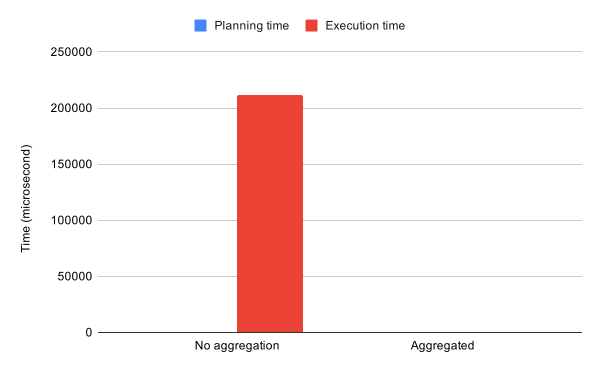
\includegraphics[width=\textwidth]{images/testing/count-local.png}
    \caption{linear scale}
\end{subfigure}%
\begin{subfigure}{0.5\textwidth}
    \centering
    \includegraphics[width=\textwidth]{images/testing/count-local-log.png}
    \caption{log scale}
\end{subfigure}
\caption{Truy vấn count trên máy local}
\end{figure}

\begin{figure}[H]
\centering
\begin{subfigure}{0.5\textwidth}
    \centering
    \includegraphics[width=\textwidth]{images/testing/count-cloud.png}
    \caption{linear scale}
\end{subfigure}%
\begin{subfigure}{0.5\textwidth}
    \centering
    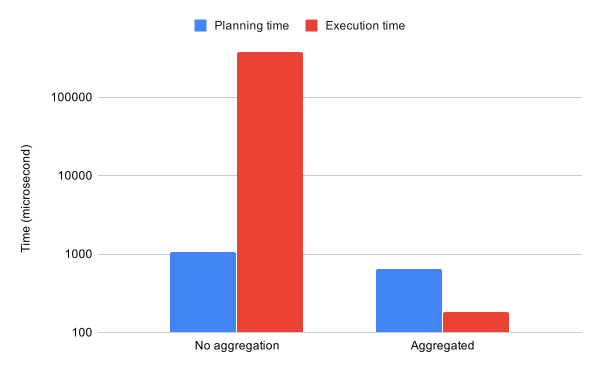
\includegraphics[width=\textwidth]{images/testing/count-cloud-log.png}
    \caption{log scale}
\end{subfigure}
\caption{Truy vấn count trên máy cloud}
\end{figure}

Đánh giá kết quả: Có thể thấy được rằng với một triệu phần tử thì
việc sử dụng trực tiếp select count là rất tốn kém, gấp rất nhiều lần
so với việc sử dụng một biến đếm riêng biệt.

\subsubsection{Truy vấn select}
\begin{figure}[H]
\centering
\begin{subfigure}{0.5\textwidth}
    \centering
    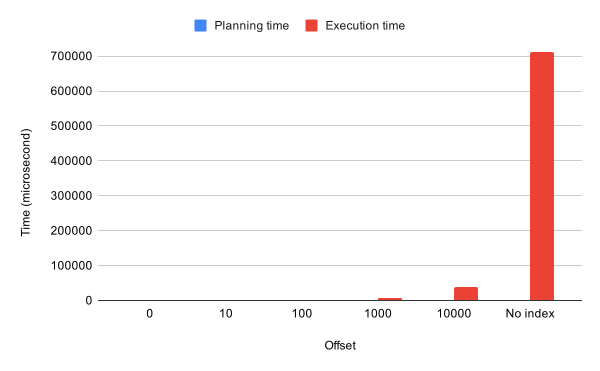
\includegraphics[width=\textwidth]{images/testing/select-local.png}
    \caption{linear scale}
\end{subfigure}%
\begin{subfigure}{0.5\textwidth}
    \centering
    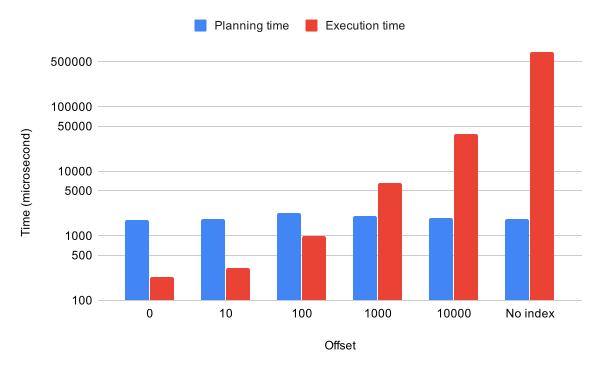
\includegraphics[width=\textwidth]{images/testing/select-local-log.png}
    \caption{log scale}
\end{subfigure}
\caption{Truy vấn select trên máy local}
\end{figure}

\begin{figure}[H]
\centering
\begin{subfigure}{0.5\textwidth}
    \centering
    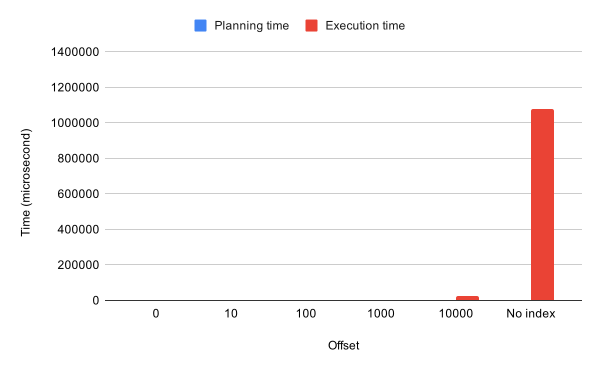
\includegraphics[width=\textwidth]{images/testing/select-cloud.png}
    \caption{linear scale}
\end{subfigure}%
\begin{subfigure}{0.5\textwidth}
    \centering
    \includegraphics[width=\textwidth]{images/testing/select-cloud-log.png}
    \caption{log scale}
\end{subfigure}
\caption{Truy vấn select trên máy cloud}
\end{figure}

Đánh giá kết quả: Có thể thấy được việc sử dụng index giúp câu lệnh
select có sắp xếp được cải thiện hiệu năng hơn rất nhiều với
bảng một triệu phần tử.
Đồng thời việc tăng offset của lệnh select cũng làm tăng dần thời gian
thực thi. Việc không sử dụng index có thể làm cho thời gian một câu lệnh
select lên đến 1s.

\subsection{Kiểm thử hiệu năng REST API}
Với bài kiểm thử hiệu năng REST API cho ứng dụng chạy trên
Microsoft Azure, ngoài việc sử dụng AKS để chạy các server
của ứng dụng thì chúng tôi sử dụng thêm một dịch vụ
khác là Container Instance để chạy các request và đo
đạc thời gian.
\begin{figure}[H]
\centering
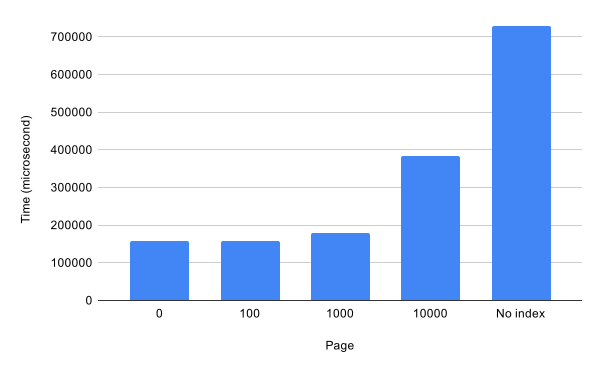
\includegraphics[width=10cm]{images/testing/view-local.png}
\caption{Hiệu năng REST API trên máy local (no aggregation)}
\end{figure}

\begin{figure}[H]
\centering
\begin{subfigure}{0.5\textwidth}
    \centering
    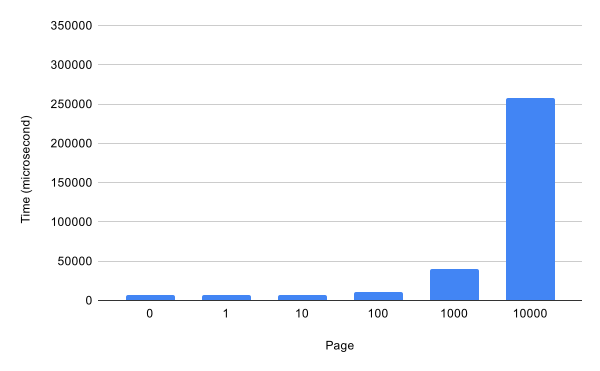
\includegraphics[width=\textwidth]
    {images/testing/view-aggregated-local.png}
    \caption{linear scale}
\end{subfigure}%
\begin{subfigure}{0.5\textwidth}
    \centering
    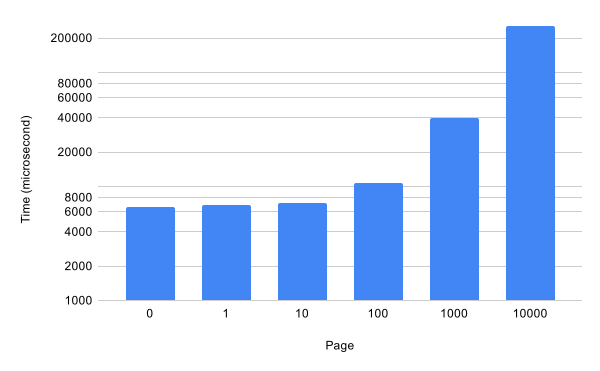
\includegraphics[width=\textwidth]
    {images/testing/view-aggregated-local-log.png}
    \caption{log scale}
\end{subfigure}
\caption{Hiệu năng REST API trên máy local (aggregated)}
\end{figure}

\begin{figure}[H]
\centering
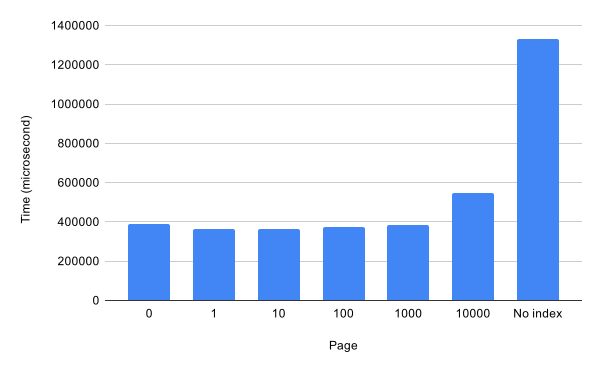
\includegraphics[width=10cm]{images/testing/view-cloud.png}
\caption{Hiệu năng REST API trên máy cloud (no aggregation)}
\end{figure}

\begin{figure}[H]
\centering
\begin{subfigure}{0.5\textwidth}
    \centering
    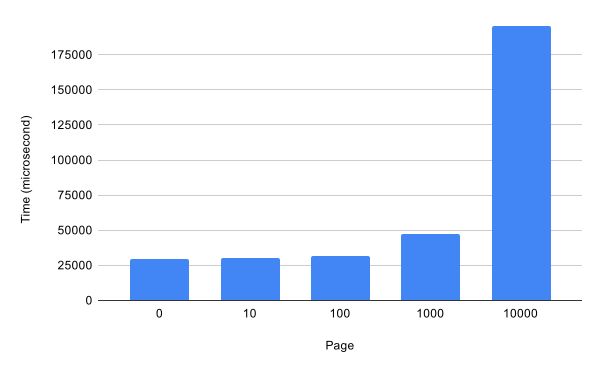
\includegraphics[width=\textwidth]
    {images/testing/view-aggregated-cloud.png}
    \caption{linear scale}
\end{subfigure}%
\begin{subfigure}{0.5\textwidth}
    \centering
    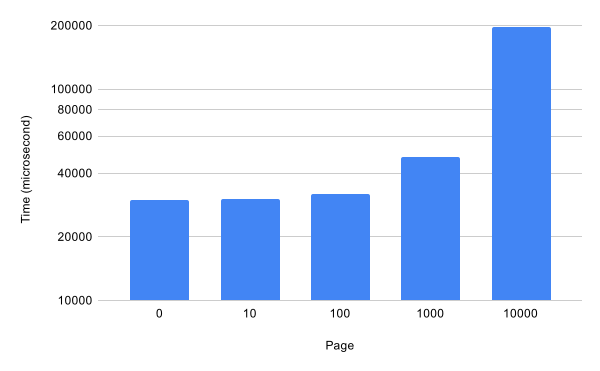
\includegraphics[width=\textwidth]
    {images/testing/view-aggregated-cloud-log.png}
    \caption{log scale}
\end{subfigure}
\caption{Hiệu năng REST API trên máy cloud (aggregated)}
\end{figure}

Đánh giá kết quả: Có thể thấy ảnh hưởng của việc sử dụng
trực tiếp lệnh select count lên tốc độ của REST API là rất lớn.
Tốc độ chậm của lệnh select count khiến cho REST API không thể kết thúc
dưới 100ms.

\section{Kiểm thử sức chịu tải (stress testing)}
Với bài toán kiểm thử sức chịu tải, chúng tôi cho đồng thời
một số lượng luồng chạy và gửi request lên server và
tính thời gian hoàn thành. Số lượng luồng tương ứng
là 1, 10 và 100.

\begin{figure}[H]
\centering
\begin{subfigure}{0.5\textwidth}
    \centering
    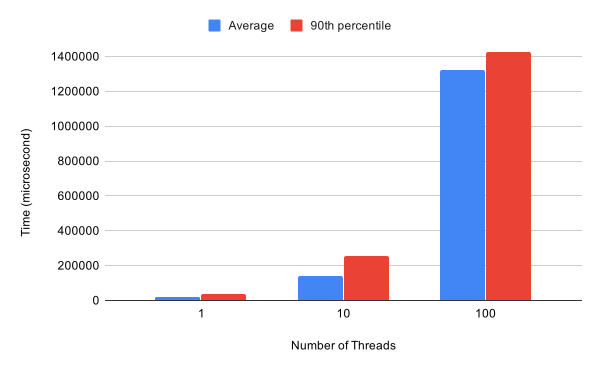
\includegraphics[width=\textwidth]
    {images/testing/stress-add-inventory-item.png}
    \caption{linear scale}
\end{subfigure}%
\begin{subfigure}{0.5\textwidth}
    \centering
    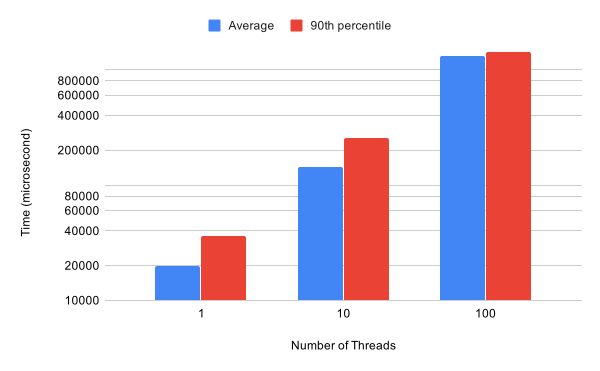
\includegraphics[width=\textwidth]
    {images/testing/stress-add-inventory-item-log.png}
    \caption{log scale}
\end{subfigure}
\caption{Stress test thêm inventory item trên máy local}
\end{figure}

\begin{figure}[H]
\centering
\begin{subfigure}{0.5\textwidth}
    \centering
    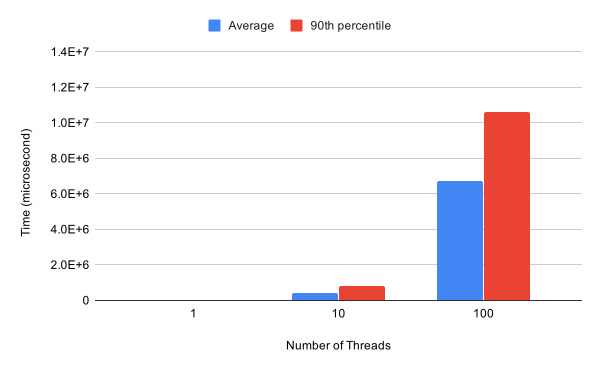
\includegraphics[width=\textwidth]
    {images/testing/stress-add-inventory-item-cloud.png}
    \caption{linear scale}
\end{subfigure}%
\begin{subfigure}{0.5\textwidth}
    \centering
    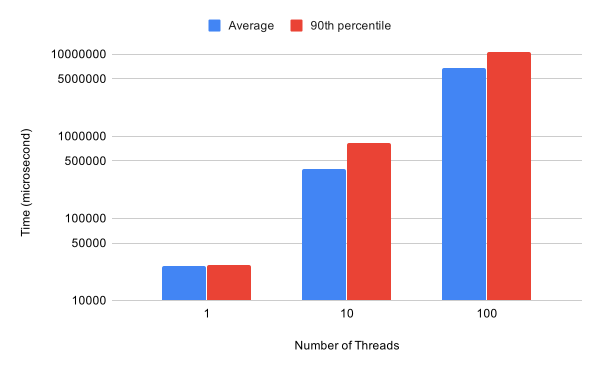
\includegraphics[width=\textwidth]
    {images/testing/stress-add-inventory-item-cloud-log.png}
    \caption{log scale}
\end{subfigure}
\caption{Stress test thêm inventory item trên máy cloud}
\end{figure}

Đánh giá kết quả: Khi tăng số request chạy đồng thời thì thời gian
chạy của các request cũng tăng lên do server chỉ có thể xử lý
đồng thời được một số lượng hữu hạn các request, các request vượt
giới hạn dó sẽ phải đợi request trước đó hoàn thành.
